\documentclass[fleqn,10pt]{article} % Document font size and equations flushed left
\usepackage{color}
\usepackage{graphicx}
\newcommand{\todo}[1]{}
\renewcommand{\todo}[1]{{\color{red} TODO: {#1}}}

%
%   BIBLIOGRAPHY
%
\usepackage{cite}
%----------------------------------------------------------------------------------------
%	COLUMNS
%----------------------------------------------------------------------------------------

\setlength{\columnsep}{0.55cm} % Distance between the two columns of text
\setlength{\fboxrule}{0.75pt} % Width of the border around the abstract

%----------------------------------------------------------------------------------------
%	COLORS
%----------------------------------------------------------------------------------------

\definecolor{color1}{RGB}{0,0,90} % Color of the article title and sections
\definecolor{color2}{RGB}{0,20,20} % Color of the boxes behind the abstract and headings

%----------------------------------------------------------------------------------------
%	HYPERLINKS
%----------------------------------------------------------------------------------------

\usepackage{hyperref} % Required for hyperlinks
\hypersetup{hidelinks,colorlinks,breaklinks=true,urlcolor=color2,citecolor=color1,linkcolor=color1,bookmarksopen=false,pdftitle={Title},pdfauthor={Author}}

%----------------------------------------------------------------------------------------
%	ARTICLE INFORMATION
%----------------------------------------------------------------------------------------
\title{DeepRTS: Flexible Deep Learning environment for Real Time Strategy Games}
\date{\today}
\author{Per-Arne Andersen \and Morten Goodwin \and Ole-Christoffer Granmo}


% Deep Learning --- Reinforment Learning --- Neural Network --- Deep-Q-Network --- Tree Search --- Monte Carlo Methods --- POMDP --- MDP --- Real Time Strategy



\begin{document}
\flushbottom % Makes all text pages the same height
\maketitle % Print the title and abstract box
%----------------------------------------------------------------------------------------
%	ABSTRACT
%----------------------------------------------------------------------------------------
\begin{abstract}
We propose a Deep learning environment, \textit{\textbf{DeepRTS}} for edge research in the field of artificial intelligence. 
Games are a excellent tool for creating novel AI techniques which can be adopted to real world scenarios. The proposed environment is a high performance, real-time strategy game with several API gateways for artificial intelligence research. RTS games are known to have a high state branching factor. This forces proposed algorithms to have a high discover rate, or a technique to easily locate important features the state space. This work present results of Monte-Carlo Tree Search and Deep Q-Learning applied to the environment. An survey of applicable algorithms for solving RTS is also outlined to create a future work roadmap for the learning environment.
\end{abstract}
%----------------------------------------------------------------------------------------

\newpage

\tableofcontents % Print the contents section

\thispagestyle{empty} % Removes page numbering from the first page
\newpage
%----------------------------------------------------------------------------------------
%	ARTICLE CONTENTS
%----------------------------------------------------------------------------------------

\section{Introduction} % The \section*{} command stops section numbering
% What the problem is (Does not exist anything between microRTS and SC2)
There exist no Real-Time strategy game (RTS) simulator environment that support a sufficiently challenging environment for complex deep learning algorithms. MircoRTS is an excellent tool for testing novel AI techniques at a basic level. But is limited to those simple scenarios. Starcraft 2 is a game by Blizzard Entertainment, and is a full fledged game with complex game mechanics. DeepRTS attempts to fill the gap between MicroRTS and Starcraft 2 by enabling research at a range of complexity levels, from the most basic scenarios, to scenarios which are close to matching Starcraft 2.
\\
\\
% Why it is important and difficult
AI today are still at a primitive stage. It can handle complex tasks but usually only in a specific area. Health, Military, Finances and Education are examples of institutions which can benefit from artificial intelligence. It is a important field of research which can greatly impact quality of human lives. Real world scenarios are very complex, and it is therefore important to test critical algorithms in an simulated environment first. Computer games are a great way of testing algorithms to measure the performance before adopting it to the real world.
\\
\\
% 1 https://en.wikipedia.org/wiki/Game_complexity
% 2 https://en.wikipedia.org/wiki/AlphaGo#Hardware
% 3 (http://www.cs.mun.ca/~dchurchill/pdf/starcraft_survey.pdf)
% Why is it hard
RTS are a genre which features real-time events from multiple players. This renders current methods of state-space searching almost impossible with the technology today. Starcraft 2, worlds most popular RTS game are expected to be one of the biggest challenge of reinforcement learning because of the huge search-space. Its hard to measure its maximum state-space, but one are certain that it expands beyond $10^{1024}$. An AI algorithm must be able to understand and construct abstractions to the state-space in order to drastically reduce its search space.
Controlling an agent in an environment where the sensory data is sparse, abstract and hard to interpret directly, is one of the most challenging tasks yet to be solved in the realm of reinforcement learning (RL). RL is an area of machine learning, where the agent directly interacts  with the environment to learn a \textit{policy}. This policy determines how the agent reacts to its environment, and does a action based on this.
Challenges arises when the problem becomes complex, such as large state and action spaces. To give an idea of what a large state space is we can estimate chess to be $10^{47}$ [1] , the game of Go to be $10^{170}$ [1]. The game of Go, was until recently a impossible problem because of hardware limitation, but with todays proccessing power, this became possible. But Go is still not possible to beat using a regular computer, as it required google to construct a distributed machine with 1920 CPUs and 280GPUs having 64 concurrent threads  searching for the next best move. [2]
\\
\\
% Why hasn't it been solved before? (Or, what's wrong with previous proposed solutions? How does mine differ?)
MicroRTS is a excellent RTS simulator, but does not enough content to push deep learning further. It can easily be mastered by DeepMind's Deep Q-Network and variations of this algorithm can outperform human play. It was designed with tree-search algorithms in mind, but it suffers from some limitations in performance due language choices. DeepRTS attempts to solve these topics by being a performance oriented engine written in pure C++. It have abstraction layers which allows for all kinds of research in the machine learning realm, with deep learning as primary research field.
\\
\\
% What are the key components of my approach and results? Also include any specific limitations.
This report presents the game simulator \textit{DeepRTS} with initial results in Monte Carlo Tree-Search and the novel algorithm Deep Q-Learning from Google DeepMind. \todo{Ka mer ska eg skriva her da}
%------------------------------------------------
\section{State of the art} % The \section*{} command stops section numbering
Deep Learning is a field which has a fast paced research speed. Google, Facebook, Facebook and so on are constantly pushing the borders of deep learning to master the ultimate goal of \textit{superintelligence}. One of the biggest achievements in deep learning in recent time is Alpha GO, which in march 2016 defeated 9-dan Lee Sedol \cite{Silver_2016}. \textit{Playing Atari with Deep Reinforcement Learning} is a novel algorithm based on Q-Learning combined with Neural Network (DQN) \cite{DBLP:journals/corr/MnihKSGAWR13}. Current state-of-the-art is DeepStack, a recent general-purpose algorithm which attempts to solve numerous imperfect information games like Texas no-limit Texas hold’em \cite{DBLP:journals/corr/MoravcikSBLMBDW17}.


\section{Real-Time Strategy Games}
RTS is a subgenre of strategy games where each player must a base, gather resources and construct an army in order to defeat their opponents. In contrast to \textit{Chess}, RTS games differs by allowing \textit{simultaneous actions} meaning that all players can issue actions at the same time. The real-time aspect of RTS games increases the difficulty level because it encourage players to perform actions frequently, often as frequent as 50 ms. R


\begin{itemize}
    \item What is an RTS?
    \item Why is it hard?
    \item What exists? (Other research, microRTS.. etc)
    \item Which algorithms are worth trying out? any algorithms that looks promising? DeepNNs?, MCTS?
    \item Test
\end{itemize}


\section{DeepRTS}
RTS is one of the most difficult problems to solve using machine learning [NEED SOURCE]. Continuous state-space with huge action spaces requires computational power beyond the capabilities of current hardware [NEED SOURCE]. In order to solve Star Craft 2, \textbf{DeepRTS} is a suited problem to start at.


\begin{figure}[ht]\centering
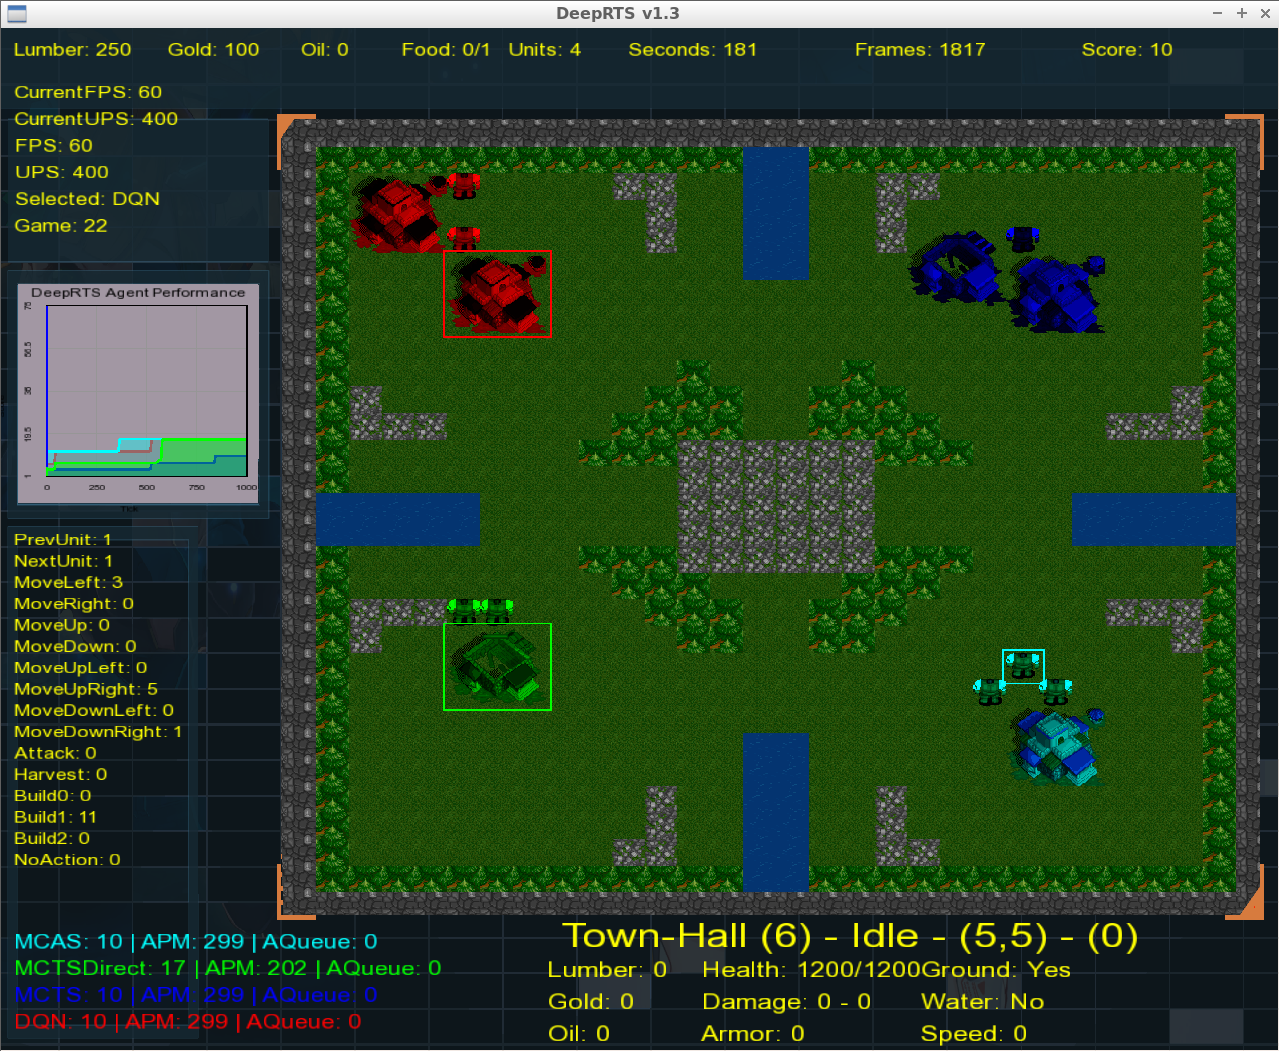
\includegraphics[width=\linewidth]{deep_rts}
\caption{DeepRTS Simulator}
\label{fig:results}
\end{figure}

The objective of playing DeepRTS is to build a base consisting of an Town-Hall and then expand the base in order to gain military power to defeat the opponents. Each of the players start with a worker. Workers can build and gather resources in the game to improve the players base.   [NEED REVISING, skriver så en tulling]. The game consist of two main termonologies, \textit{Micro} and \textit{Macro} management. In order to win, the player with the best ability to both micro and macro mange their resources are most likely to win. [OMMMG REVISE]

DeepRTS was specifically developed for high-performance simulation for the RTS genre. It is developed in C++ with API for Python, websockets, LUA and ZeroMQ. It focuses on being flexible in configuration to allow for development of different AI approaches, i.e reinforcement learning and unsupervised learning. The simulator also features a python version which can be used with Gym, however it does not perform as good as the C++ implementation, but it is well suited for GPU based machine learning.

The game interface attempts to display all of the important statistics meanwhile a game is ongoing. This being \textit{action execution distribution}, player resources, player scores and a live performance graph.
Additionally the game have multiple hot-keys for moderating game-speed and graphics. A Detailed list of these hot-keys can be found by pressing the \textit{G}-hotkey. 

One of its major features is that it allow up to 16 players. At current level of AI, a reasonable goal is 3 players. This is because it eliminates possibility for regular min-max strategies [NEED SOURCE]. Some algorithms have been developed for basic game-play, specifically algorithms based on \textit{Monte-Carlo Methods}, these will be thoroughly discussed in the upcoming chapters.
The goal of DeepRTS is to improve productivity and the understanding of artificial intelligence, and making it possible to further expand towards a super intelligent AI.

%------------------------------------------------

\section{Algorithms}

\subsection{DQN}
Q-Learning is a strong family of algorithms used to determine which state



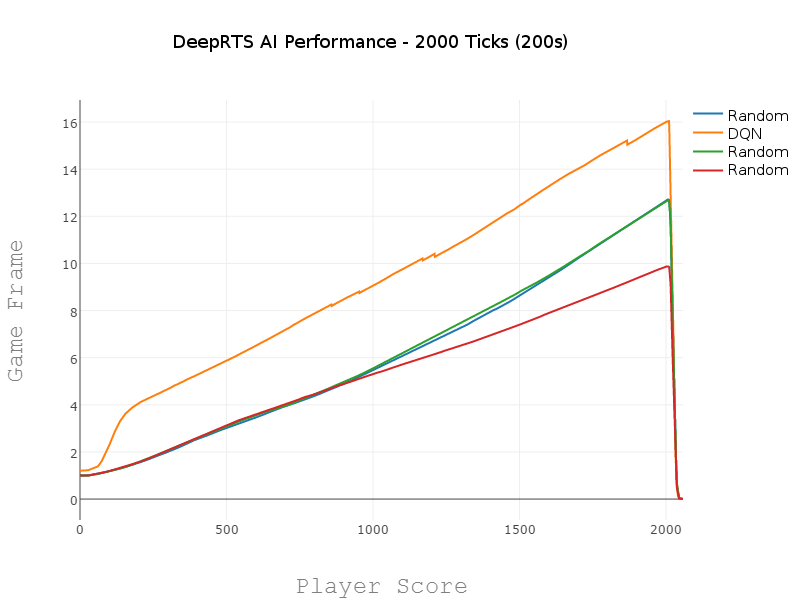
\includegraphics[width=\linewidth]{3000.png}
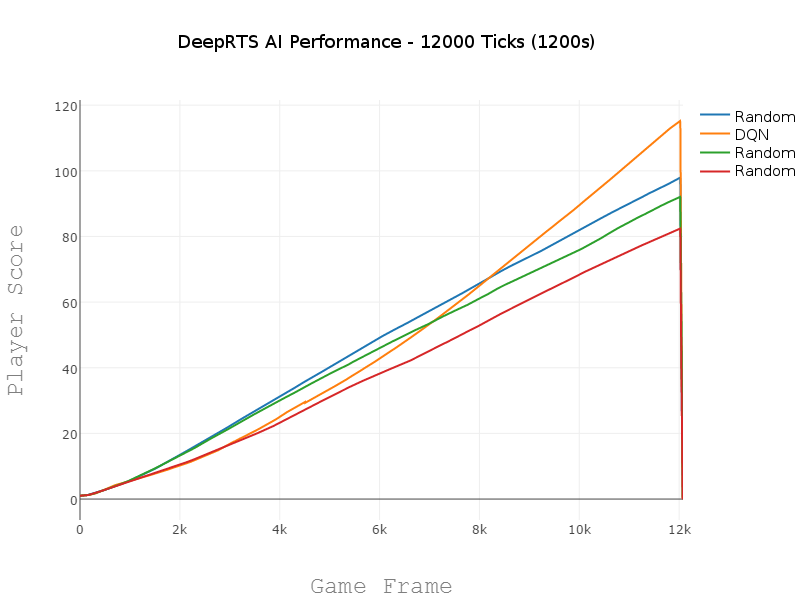
\includegraphics[width=\linewidth]{12000.png}


\subsection{Monte-Carlo Methods}
Monte-Carlo methods (MCM) works by using random-sampling to attempt to find an optimal solution. Eventually an optimal state will be found given an indefinite time budget. Monte-Carlo Tree search is the algorithm of research covered here, with some alterations which branch into a new algorithm \textit{Monte-Carlo Graph Search}.
Tree-Search algorithms are widely used in chess and other turn-based games, and perform well in scenarios where the time budget is high. The more computational time, the bigger branching scope are being discovered and thus yielding a high expertise level.
In DeepRTS MCM is challenge becuase it has yet to perform well in games with more than two players \todo{[NEED SOURCE]}. DeepRTS is also an complex game where state-space is beyond the known scope of success for this algorithm genre. Specifically, \textit{Monte-Carlo Direct Approach} shown good results which may be an indication that high-level abstractions can improve performance of tree-seach algorithms [NEED SOURCE]
\\
\\
In DeepRTS, all MCM methods have a finite time-budget set to \textbf{18} milliseconds. Additionally all of the algorithms are configured with an depth-limit of \textbf{10}. 
Each algorithm uses a unique heuristic for selecting the optimal action per cycle, and these will be discussed thoroughly in the upcoming subsections.
\subsubsection*{Upper Confidence Bounds}
blablablac

\subsubsection*{UCB Action Search}
blablala

\subsubsection*{Direct Greedy Approach}
blablabla

\subsubsection*{Graph Search}

\section{Theoretical Aproaches}
\begin{itemize}
    \item Algorithms that may work
\end{itemize}

\section{Results}

%------------------------------------------------
\phantomsection
\section*{Acknowledgments} % The \section*{} command stops section numbering

\addcontentsline{toc}{section}{Acknowledgments} % Adds this section to the table of contents

So long and thanks for all the fish \cite{Figueredo:2009dg}.

%----------------------------------------------------------------------------------------
%	REFERENCE LIST
%----------------------------------------------------------------------------------------
\phantomsection
\bibliographystyle{unsrt}
\bibliography{sample}

%----------------------------------------------------------------------------------------

\end{document}
